
\section{Dynamics of Composed Particles}


In nature it is easy to find systems in which the interactions also depends on the size and the shape of the particles (e.g. molecules, crystals, landslides...). To approximate the motion, the interaction and the development of such systems one has to consider the shape and the composition of its composing particles. We will therefore start with the model of rigid bodies, and then relax the condition of rigidity a bit. This implies the following important consideration: it would be an oversight if we would simulate at energies at which the bonds that compose the particles are destroyed. 


\vspace{0.1cm}
\noindent
\begin{minipage}{\textwidth}
\begin{minipage}{.6\textwidth}%
Given the assumption that the bonds are stable in the simulated energy regime, there is a wide range of situations in which these methods are very useful. As an example, at room temperature the  air molecules are not going to break up in their components. The atoms that compose the molecules will also not break up if not in very special situations (ionization in the higher atmosphere or on stars' surfaces, particle accelerators, etc.). As a practical example, consider a water molecule ($H_2O$). In this case, the distance and angles between the atoms are fixed.
 \end{minipage}%
\hfill
\begin{minipage}{.4\textwidth}%
  \centering
  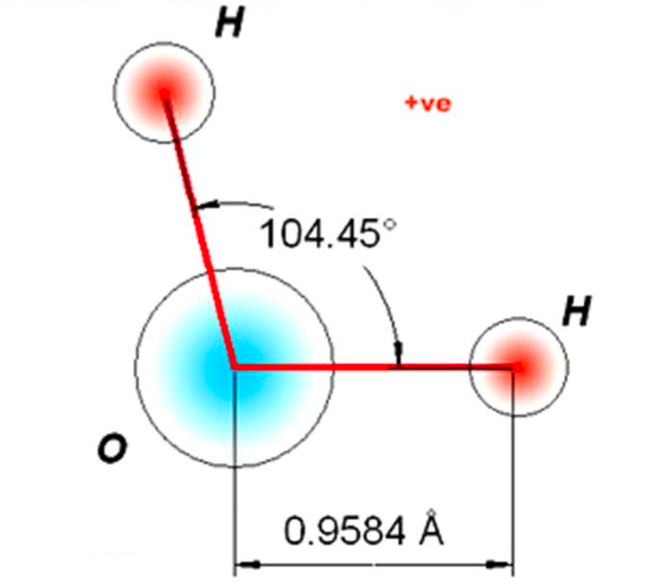
\includegraphics[width=\textwidth]{pics/water}
  %\captionof{figure}{Comparison of the precision in the Verlet method and the predictor-corrector of various order.}
  \label{fig:water}
\end{minipage}
\end{minipage}
\vspace{0.1cm}

There are two main methods applied to such a situation:
\begin{itemize}
\item Lagrange multipliers 
\item Rigid body approximation (good for arbitrary shapes)
\end{itemize}



\subsection{Lagrange multipliers}

\citet{lagrange} were one of the first to propose an extra force term in the equations of motion to impose the constraints given by a speficic shape of the composed particle (e.g. a molecule):

\begin{equation}
m_i\ddot{\vec{x}}_i = \underbrace{f_i}_{\text{external interaction}} + \underbrace{\vec{g}_i}_{\text{internal constraints}}
\end{equation}

We can impose constraining forces that will enforce the geometric arrangement of the molecules, e.g. certain distances $d_{1,2}$ and $d_{2,3}$ between atoms. In this case, the constraint forces are proportional to the difference of the actual and the desired distance of the particles. We can define a potential:

$$
\chi_{1,2} \equiv r^2_{1,2} -d^2_{1,2} \overset{\text{rest}}{=} 0
$$
\begin{equation}
\chi_{2,3} \equiv r^2_{2,3} -d^2_{2,3} \overset{\text{rest}}{=} 0
\end{equation}

The equality to zero only holds if the particles have a distance ($r_{ij}$)  equal to the chosen rest position $d_{ij}$. With $r_{ij}\equiv \abs{\vec{r}_{i,j}}$, $\vec{r}_{i,j} \equiv \vec{x}_{i}  -\vec{x}_{j} $ one can obtain
  $$ \vec{g}_k = \frac{\lambda_{1,2} }{2} \vec{\nabla} _{\vec{x}_k} \chi_{1,2}+
                   \frac{\lambda_{2,3} }{2} \vec{\nabla} _{\vec{x}_k} \chi_{2,3}
 $$ we can define the Lagrange multipliers, $\lambda_{1,2}$ and $\lambda_{2,3}$, yet to be determined. We will compute these multipliers by imposing constraints. The force is then obtained by the gradient of the potential:
 \begin{equation}
 \Rightarrow \vec{g}_1 = \lambda_{1,2} \vec{r}_{1,2}, \hspace{0.4cm} 
\vec{g}_2 = \lambda_{2,3} \vec{r}_{2,3} - \lambda_{1,2} \vec{r}_{1,2}, \hspace{0.4cm} 
\vec{g}_3 = - \lambda_{2,3} \vec{r}_{2,3}.
\label{eq:lagrange_forces}
\end{equation}
 This is simply a linear spring with a  yet to be determined spring constant $\lambda$. To obtain the values of $\lambda$, the Verlet algorithm is executed in two steps: first we will compute the forces on the molecules:
 $$
\tilde{\vec{x}}_i \kl{t+\Delta t} = 2\vec{x}_i  - \vec{x}_i\kl{t-\Delta t} + \Delta t ^2 \frac{f_i}{m_i} 
$$ 
and then we correct the value using the above the constraints:
$$
\vec{x}_i \kl{t+\Delta t} = \tilde{\vec{x}}_i \kl{t+\Delta t} + \Delta t ^2 \frac{\vec{g}_i}{m_i} 
$$
We can insert \eqref{eq:lagrange_forces} into the last expression to find the updated positions:

\begin{align}
\vec{x}_1 \kl{t+\Delta t} &= \tilde{\vec{x}}_1 \kl{t+\Delta t} + \Delta t ^2 \frac{\lambda_{1,2}}{m_2} \vec{r}_{2,3}\kl{t}\\
\vec{x}_2 \kl{t+\Delta t} &= \tilde{\vec{x}}_2 \kl{t+\Delta t} + \Delta t ^2 \frac{\lambda_{2,3}}{m_1} \vec{r}_{1,2}\kl{t} -  \Delta t ^2 \frac{\lambda_{1,2}}{m_2} \vec{r}_{1,2}\kl{t}\\
\vec{x}_3 \kl{t+\Delta t} &= \tilde{\vec{x}}_3 \kl{t+\Delta t} + \Delta t ^2 \frac{\lambda_{2,3}}{m_3} \vec{r}_{2,3}\kl{t}
\end{align}
With these expressions, we can obtain now $\lambda_{1,2}$ and $\lambda_{2,3}$ by inserting them into the constraint condition:

$$
\abs{\vec{x}_1 \kl{t+\Delta t} - \vec{x}_2 \kl{t+\Delta t}}^2 = d_{1,2}
$$
$$
\abs{\vec{x}_2 \kl{t+\Delta t} - \vec{x}_3 \kl{t+\Delta t}}^2 = d_{2,3}
$$
$$
\Rightarrow
$$

$$
\abs{      \tilde{ \vec{x}}_1 \kl{t+\Delta t} -\tilde{  \vec{x}}_2 \kl{t+\Delta t} + \Delta t^2 \lambda_{1,2} \kl{\frac{1}{m_1} +\frac{1}{m_2}}\vec{r}_{1,2}\kl{t}  - \Delta t^2 \frac{\lambda_{2,3}}{m_2 \vec{r}_{2,3}\kl{t}}        }^2 = d_{1,2}
$$
$$
\abs{      \tilde{  \vec{x}}_2 \kl{t+\Delta t} - \tilde{ \vec{x}}_3 \kl{t+\Delta t} + \Delta t^2 \lambda_{2,3} \kl{\frac{1}{m_2} +\frac{1}{m_3}}\vec{r}_{2,3}\kl{t}  - \Delta t^2 \frac{\lambda_{2,3}}{m_2 \vec{r}_{1,2}\kl{t}}        }^2 = d_{2,3}
$$
These expressions can be solved  for $\lambda_{1,2}$ and $\lambda_{2,3}$ that can be then used to calculate the next position $\vec{x}_i\kl{t+\Delta t}$. Depending on the precision needed one can ignore the higher order terms of $\Delta t$.


\subsection{Rigid Bodies}
In the case of a rigid body (an object in which the distances of the particles composing it remain constant), particle motion can be split into translation of the center of mass and rotation of the body: the center of mass
\begin{equation}
M\vec{x}_{cm} \equiv \sum_{i=1}^n{\vec{x}_im_i}
\hspace{0.4cm}\text{with}\hspace{0.4cm} 
M\equiv \sum_{i=1}^n{m_i}
\label{eq:center_of_mass}
\end{equation}

follows the equations of motion and the rotation is given by the torque,
\begin{equation}
M\ddot{\vec{x}}_{cm} = \sum_{i=1}^n{f_i} \equiv f_{com}
\hspace{0.4cm}\text{and}\hspace{0.4cm} 
\vec{T} \equiv \sum_{i=1}^n{     \vec{d}_i \times     f_i   }
\label{eq:cof_eom}
\end{equation}
with $\vec{d}_i \equiv \vec{x}_i - \vec{x}_{cm}$.

In two dimensions  the rotation always points in the direction of the normal vector of the plane. There are therefore only three degrees of freedom: two translational and one rotational. In three dimensions there are six degrees of freedom. We well first introduce the two-dimensional case and then generalize to the three-dimensional case.

\subsubsection*{2D:}
In 2D,  the moment of inertia and the torque are given by

$$
I = \int\int_{A}{r^2 \rho \kl{r} \text{dA}}
\hspace{0.4cm}\text{and}\hspace{0.4cm} 
T = \int\int_{A}{f_t\kl{r} r \text{dA}}.
\label{eq:cof_eom}
$$
From Newton's equations one can derive the equation of motion for the rotation:
\begin{equation}
I\dot{\omega} = T.
\label{eq:eom_rot}
\end{equation}

We can calculate the time evolution of the rotation angle $\phi$ by applying the Verlet algorithm to the variable $\phi\kl{t}$:
$$
\phi\kl{t+\Delta t} = 2 \phi\kl{t} -\phi\kl{t-\Delta t} + \Delta t^2 \underbrace{ \frac{T\kl{t}}{I}}_{=\dot{\vec{\omega}}}
$$
 $$
\vec{x}\kl{t+\Delta t} = 2 \vec{x}\kl{t} -\vec{x}\kl{t-\Delta t} + \Delta t^2 M^{-1} \sum_{j\in A} {f_j\kl{t}}
 $$
 where the torque can be calculated summing over all the torques in the body: $T\kl{t} = \sum_{j\in A} \ekl{    f^y_j\kl{t} d^x_j\kl{t} -  f^x_j\kl{t} d^y_j\kl{t}     }$. 
 

\subsubsection*{3D:}
If we expand our model to the third dimension, we will see that the computation is not as simple as on a plane where the torques and angular momenta always point in the same direction. As in classical mechanics we define the angular momentum as
$$
\vec{l} \equiv \sum_{i=1}^n{m_i\vec{d}_i \times \vec{v}_i} 
= \sum_{i=1}^n{m_i\vec{d}_i \times \kl{\vec{d}_i \times \vec{\omega}}} 
= \sum_{i=1}^n {m_i   \kl{\vec{d}_i    \kl{\vec{d}_i \vec{\omega}}   -\vec{d}_i^{\,\,2}\vec{\omega} }  }     
= \mat{I} \vec{\omega}.
$$
With this definition the equation of motion is
$$
\dot{\vec{l}} = \mat{I}\dot{\vec{\omega}} = \vec{T}
$$  
where $\mat{I}$ is the \emph{tensor of inertia}. The tensor of inertia describes the motion of rigid bodies and it can be generally written as
$$
\mat{I} = \sum _{i=1}^n {m_i \kl{  \vec{d}_i^{\,\,T}  \bigotimes    \vec{d}_i   -\vec{d}_i^{\,\,2} \vec{l}\,\,    }       }
$$
 This tensor can be brought into a diagonal form by transforming the coordinate system into a body-fixed coordinate system with origin in the center of mass and basis vectors pointing in the directions of the eigenvectors of the tensor. The basis transformation can be written with a matrix $\mat{A}$:
 \begin{equation}
\underbrace{ \vec{e}^{\,\,b} }_{b.c.s.}= \underbrace{ \mat{A}\vec{e}^{\,l} }_{l.c.s.}
\label{eq:transf_mat}
\end{equation}

 $$
\dot{\vec{l}}^{\,\,l} = \vec{T}^{\,l} 
\hspace{0.4cm} \Rightarrow \hspace{0.4cm}
\dot{\vec{l}}^{\,\,b} + \vec{\omega}^b\times\vec{l}^{\,\,b} = \mat{I} \dot{\vec{\omega}}^b + \vec{\omega}^b \times \vec{l}^{\,\,b} = \vec{T}^{\,b}
\hspace{0.4cm} \Leftrightarrow \hspace{0.4cm}
\mat{I} \dot{\vec{\omega}}^b  = \vec{T}^{\,b} - \vec{\omega}^b \times \vec{l}^{\,\,b}
$$

Without derivation, this can be then transformed into a system of equations

\begin{align}
\dot{\vec{\omega}}_x^b &= \frac{\vec{T}^b_x}{I_{xx}} + \kl{\frac{\mat{I}_{yy}-\mat{I}_{zz}}{\mat{I}_{xx}}   } \vec{\omega}^b_y\vec{\omega}^b_z \\
\dot{\vec{\omega}}_y^b &= \frac{\vec{T}^b_y}{I_{yy}} + \kl{\frac{\mat{I}_{zz}-\mat{I}_{xx}}{\mat{I}_{yy}}   } \vec{\omega}^b_z\vec{\omega}^b_x \\
\dot{\vec{\omega}}_z^b &= \frac{\vec{T}^b_z}{I_{zz}} + \kl{  \frac{\mat{I}_{xx}-\mat{I}_{yy}}{\mat{I}_{zz}}   } \vec{\omega}^b_x\vec{\omega}^b_y
\end{align}
with the tensor of inertia being diagonal in the body frame: 
$$\mat{I} = \begin{pmatrix}
 I_{xx} & 0 & 0\\
 0 & I_{yy} & 0 \\
 0 & 0 & I_{zz}  
\end{pmatrix}. $$ 
As we can see, the diagonal form of the tensor of inertia comes with the cost of one added term. Together with \eqref{eq:transf_mat} we can compute the angular velocities:

$$
\vec{T}^{\,l} = \sum_{i=1}^n   {\vec{d}_i \times f_i} 
\hspace{0.4cm} \Rightarrow \hspace{0.4cm}
\vec{T}^b = \mat{A}\vec{T}^l
$$


\begin{align}
\vec{\omega}^b_x \kl{t+\Delta t}  &= \vec{\omega}^b_x \kl{t} + 
\Delta t \frac  {\vec{T}^b_x \kl{t} }{I_{xx}} + \Delta t \kl{\frac{\mat{I}_{yy}-\mat{I}_{zz}}{\mat{I}_{xx}}   } \vec{\omega}^b_y\vec{\omega}^b_z \\
\vec{\omega}^b_y \kl{t+\Delta t} &= \vec{\omega}^b_y \kl{t} + 
\Delta t \frac  {\vec{T}^b_y \kl{t} }{I_{yy}} + \Delta t \kl{\frac{\mat{I}_{zz}-\mat{I}_{xx}}{\mat{I}_{yy}}   } \vec{\omega}^b_z\vec{\omega}^b_x \\
\vec{\omega}^b_z \kl{t+\Delta t} &= \vec{\omega}^b_z \kl{t} + 
\Delta t \frac  {\vec{T}^b_z \kl{t} }{I_{zz}} + \Delta t \kl{\frac{\mat{I}_{xx}-\mat{I}_{yy}}{\mat{I}_{zz}}   } \vec{\omega}^b_x\vec{\omega}^b_y
\end{align}
From these expressions  and \eqref{eq:transf_mat}  one can easily obtain the angular velocity in the laboratory frame:
$$
\vec{\omega}^l \kl{t+\Delta t} = \mat{A}^T \vec{\omega}^b\kl{t+\Delta t}.
$$
Since the particles are moving all the time, the transformation matrix in equation \eqref{eq:transf_mat} is not constant. We therefore have to find an efficient way to determine and update $\mat{A}$ at every step. This can be done using either Euler angles and quaternions. The following will be only a summary of the derivation, since these topics are generally treated in classical mechanics.



\subsubsection*{Euler angles:}
We will begin by defining the transformation matrix for a rotated frame of reference. We assume that the transformation matrix for a rotation around the Euler angles is already known. There are a huge number of different conventions. One way to represent an arbitrary rotation is through the following combination of rotations:
$$
\mat{A} = 
\begin{pmatrix}
 \cos{\Psi}  & -\sin{\Psi} & 0 \\
 \sin{\Psi} & \cos{\Psi} &0\\
 0 & 0 & 1   
\end{pmatrix} 
\cdot
\begin{pmatrix}
 1 & 0 & 0 \\
0 & \cos{\Theta} & -\sin{\Theta} \\
 0 & \sin{\Theta} & \cos{\Theta}  
 \end{pmatrix} 
\cdot
\begin{pmatrix}
 \cos{\Phi} & -\sin{\Phi} & 0  \\
 \sin{\Phi} & \cos{\Phi}  & 0  \\
 0 & 0 & 1  
\end{pmatrix} 
$$
\begin{equation}
.
 \label{eq:horr_mat}
\end{equation}

$$
= 
\begin{pmatrix}
 \cos{\Phi} \cos{\Psi}  -\sin{\Phi}\sin{\Psi}-\cos{\Theta}   & \sin{\Phi}\cos{\Psi} + \cos{\Phi}\cos{\Theta}\sin{\Psi} & \sin{\Theta}\sin{\Psi}\\
 -\cos{\Phi}\sin{\Psi} +\sin{\Phi}\cos{\Theta}\cos{\Psi} & -\sin{\Phi}\sin{\Psi} + \cos{\Phi}\cos{\Theta}\cos{\Psi} & \sin{\Theta}\cos{\Psi} \\
 \sin{\Phi}\sin{\Theta} & -\cos{\Phi}\sin{\Theta} & \cos{\Theta}
% \label{eq:horr_mat}
\end{pmatrix} .
$$

The take-home message here is that an arbitrary rotation can assume a very nasty form which is everything but well suited for an efficient implementation. One has to keep in mind that this operation has to be done for every particle and for every time step, making this approach prohibitive for what concerns the time consumption. One can also find analytical relations to the angular velocities
\begin{align}
\dot{\Phi} &= -\omega^l_x \frac{\sin{\Phi}\cos{\Theta}}{\sin{\Theta}} + \omega^l_y \frac{\cos{\Phi}\cos{\Theta}}{\sin{\Theta}} + \omega^l_z  \\
\dot{\Theta} &= -\omega^l_x\cos{\Theta} + \omega^l_y \sin{\Phi}  \\
\dot{\Phi} &= \omega^l_x \frac{\sin{\Phi}}{\sin{\Theta}} - \omega^l_y \frac{\cos{\Phi}}{\sin{\Theta}} 
\label{eq:ang_veloc}
\end{align}
which again are not very suitable for computation. Furthermore, one can see that this representation also has singularities, since we are dividing by $\sin{\Theta}$. We therefore have to find alternative expressions for the rotational motion.

\subsubsection*{Quaternions:}
Daniel Evans, a professor in Canberra, Australia, came up with a trick to optimize the computation of rotational velocities \citep{evans1,evans2}. This is a rather algebraic approach, which is not at all intuitive, and we will only discuss the main steps of the method here. 

Quaternions are a generalization of complex numbers, where four basis vectors span a four-dimensional space. By defining

\begin{align}
q_0 &\equiv \text{cos}\ekl{\frac{\Theta}{2}}  \text{cos}\ekl{\frac{\Phi+\Psi}{2}} \\
q_1 &\equiv \text{sin}\ekl{\frac{\Theta}{2}}  \text{cos}\ekl{\frac{\Phi-\Psi}{2}} \\
q_2 &\equiv \text{sin}\ekl{\frac{\Theta}{2}}  \text{sin}\ekl{\frac{\Phi-\Psi}{2}} \\
q_3 &\equiv \text{cos}\ekl{\frac{\Theta}{2}}  \text{sin}\ekl{\frac{\Phi+\Psi}{2}} 
\label{eq:quaternions}
\end{align}
we can represent the angles in dependence of our set of quaternions $q_i$. Note that the euclidean norm of $\vec{q}$ equals unity, therefore there are in fact only three degrees of freedom. Skipping the derivation, one can show that


$$
\mat{A}= 
\begin{pmatrix}
 q_0^2 + q_1^2 -q_2^2 -q_3^2  & 2\kl{q_1q_2+q_0q_3}  & 2\kl{q_1q_3-q_0q_2} \\
 2\kl{q_1q_2-q_0q_3}  & q_0^2 -q_1^2 +q_2^2 -q_3^2 &  2\kl{q_2q_3+q_0q_1} \\
  2\kl{q_1q_3+q_0q_2} &  2\kl{q_2q_3+q_0q_1}  & q_0^2 -q_1^2 -q_2^2 +q_3^2
\end{pmatrix} 
$$
We now have a closed form to represent our rotation, without having to calculate any products involving $\sin{x}$ and $\cos{x}$. This is by order of magnitudes faster than the expression in \eqref{eq:horr_mat}. It is a matter of algebra showing that


$$
\begin{pmatrix}
 \dot{q}_0\\
 \dot{q}_1\\
  \dot{q}_2\\
   \dot{q}_3
   \end{pmatrix} 
= \frac{1}{2}
\begin{pmatrix}
 q_0 & - q_1 &  -q_2 & -q_3 \\
 q_1 &   q_0 &  -q_3 &  q_2 \\
 q_2 &   q_3 &   q_0 & -q_1 \\
 q_3 & - q_2 &   q_1 &  q_0 
\end{pmatrix} 
\cdot
\begin{pmatrix}
 0\\
\omega^b_x\\
\omega^b_y\\
\omega^b_z\\
   \end{pmatrix} 
$$
%Since the world of quaternions and the normal euclidean space are connected by a diffeomorphism, there is always the possibility of calculating the values of the Euler angles if needed (e.g. for a plot):
If needed (e.g. for a plot) the Euler angles can be calculated from quaternions:

\begin{align}
\Phi &= \text{arctan}\ekl{ \frac{2\kl{q_0q_1+q_2q_3}}{ 1- 2\kl{q_1^2+q_2^2}}  }  \\
\Theta &= \text{arcsin}\ekl{ 2\kl{q_0q_2-q_1q_3} }  \\
\Psi &= \text{arctan}\ekl{ \frac{2\kl{q_0q_3+q_1q_2}}{ 1- 2\kl{q_2^2+q_3^2}}  }  
\label{eq:quaternions_back}
\end{align}

Mind that there is no need of calculating the Euler angles at each integration step. We can run our simulation completely with the sole use of the quaternion representation of our rigid body motion. Thus the strategy to follow is

\begin{itemize}
\item Calculate torque $T\kl{t}$ in the body frame.
\item Obtain $\omega^b\kl{t+\Delta t}$ (in quaternion representation).
\item Integrate the equation of motions (remaining in the quaternion representation).
\end{itemize}








